\chapter{State of the art}
\section{Noise Removal in Image Processing using Median [2]}

This paper was written by Monika Kohli and Harmeet Kaur. Authors research and analyze median filter. From this, the filter is compared with median and Adaptive median filter. 
\vspace{1cm}

\textbf{Types of noise}
\vspace{0.5cm}

\textbf{Impulse noise (Salt \& pepper noise):}  Used for this type of noise  Black and white dots appear in this noise so the name salt \& pepper noise. 

\

\textbf{Amplifier noise (Gaussian noise):} 
is the sum of the true pixel value and a random 

\

\textbf{Quantization noise (Uniform noise):}It is caused by quantizing the pixels to a number of discrete levels called as quantization noise. 

\

\textbf{Multiplicative noise (Speckle noise):} can be modeled by random value multiplications with pixel values of the image.



\

\textbf{Periodic noise(Stationary noise):}It is caused by interference between electronic components and appear from interference during image acquisition.
%\end{itemize}
\vspace{0.5cm}

After image noise can be classified as above, characteristics of each type are specified. They analyse algorithm of filters : Median filter, Adaptive median filter, Proposed Median Filter.  
\vspace{1cm}

%\textbf{Conclusion}

Finally, Comparison of filters when used PSNR to calculate quality of images with 3 methods : Median filter, Adaptive median filter, Proposed Median Filter. They obtained result show that the proposed method is the best. In future, result can be improved by different noise such as : Gaussian noise, Speckle noise etc
\vspace{1.5cm}

\section{The Sure-Let Approach to Image Denoising [3]}

The paper was written by Thierry Blu and Florian Luisier. It's a new approach to image denoising, based on the image-domain minimization of an estimate of the mean squared error(MSE).
\vspace{0.5cm}


A new approach to image denoising, based on the image-domain minimization of an estimate of the mean squared error: Stein’s unbiased risk estimate (SURE). The denoising process can be expressed as a linear combination of elementary denoising processes: Linear expansion of thresholds (LET). Evaluate this denoising performances by comparing PSNR. Combined 3 step above to  SURE-LET Approach.
\vspace{1cm}

%We have SURE-LET Formula as below :
%\begin{center}


%\vspace{0.5cm}
%$\displaystyle\sum_{l=1}^{K}\underbrace{F_k(y)^T F_l(y)a_l}_{[M]_{k,l}} = \underbrace{F_k(y)^Ty-\sigma^2div\left\{F_k(y)\right\}}_{[c]_k}$     
%\vspace{0.2cm}

%$$\hspace{3.5cm} for \ k = 1,2...K$$	
%\end{center}
%\begin{center}
%\hspace{3.5cm} 	$\vspace{0.3cm}\Updownarrow$ 
	

%\hspace{3.5cm}	\textbf{Ma=c} 
%\end{center}

\textbf{Result:}

\

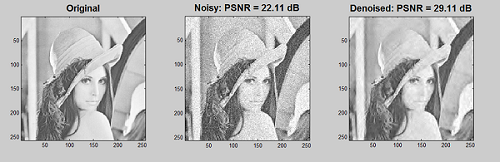
\includegraphics{surelet1.png}

\vspace{1cm}

%\textbf{Conclude:}

Follow SURE-LET program in Matlab, input MSE is compare between noisy image and original image, output MSE is compare between denoise image and original image. So they use output MSE result to table of Comparison Of The Results.
\vspace{1.5cm}

\section{Study on Methods of Noise Reduction in a Stripped Image [4]}

[Chi Chang-yan, Zhang Ji-xian, Liu Zheng-jun]

%\

Noise is one of  image quality problem in the image processing major. Noise reduction is necessary for us to do remove noise and description useful information more prominent. The Gray Value Substitution and Wavelet Transformation are methods in noise removal. Finally, MSE and PSNR are evaluated the processed image suitable in this paper.


%\subsection*{Low pass filter}
%\begin{center}
%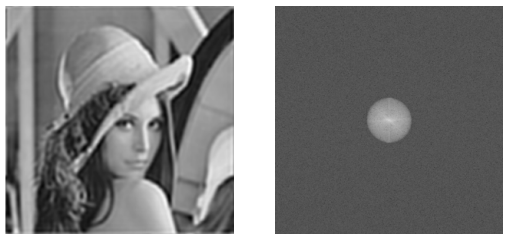
\includegraphics{lowpass.png}


%TLPF processed image and its Fourier spectrum 
%\end{center}
%Noise is high frequency signal, so they used  low pass filter to reduce it. The trapezium low pass filter (TLPF) they choose has certain advantage to smooth transition band. After processing, the image is blur than that before. Low pass filter can remove noise is meaning detailed image information is also removed. So it is not good at image which needs much spectral information. 

%\subsection*{Gray Value Substitution }
\begin{center}
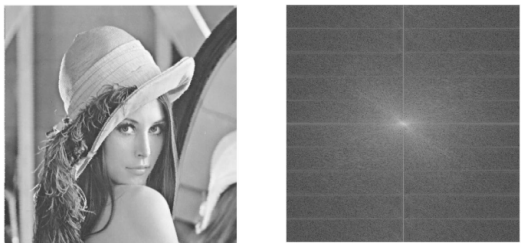
\includegraphics{gray.png}

 Image processing results of gray value substition 
\end{center}

We can see from this image, most noise line is changed and it is not affected by this method.  However, some small noise still appear, and the brightness after processing is stronger than that before. 
\vspace{2cm}
%\subsection*{Wavelet transformation }

\begin{center}
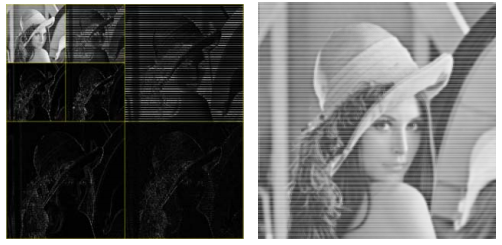
\includegraphics{wave.png}

Image decomposition using Wavelet and usual wavelet denoising result
\end{center}
Wavelet method  haven't solution remove noise in the horizontal domain, the vertical and cross part of image. Moreover this image haven't much noise so they obtain result as above. 

\
%\subsection*{Results and comparisons }

From result tables, they can see that, low pass filter can't use to remove noise. And the other two methods is relatively accepted
\vspace{1.5cm}

\section{Different Noise Types and Digital Image Processing[5]}
[Gursharan Kaur, Rakesh Kumar, Kamaljeet Kainth]


As know, image is used in various fields like medical and education. Noise appear everywhere including images. From this, noise reduction is the main focus to retain the quality of the image.This paper is review problem to types of noise and solution.

\

Types of noise: Gaussian noise, Salt and pepper noise, Poisson noise

\

Different types of linear and non-linear filters.

\

Mean Filter: Mean filter is a type of linear filter that computes average value of the corrupted image.

\

Median Filter: Median filter is a type of non-linear filter. It used to reduce the amount of intensity variation between one pixel and the other pixel.

\

%\subsection*{CONCLUSION AND FUTURE SCOPE}
In this paper, the main focus is on the denoising of the images. Techniques that are already using may not be able to find the best result so in the future they may find the techniques that provide optimum solution to the noise.
\vspace{1.5cm}

\section{Impulse Noise Reduction
methods in Digital images [6]}
[Himani Goel, Seema Rani]

\

They review this paper about denoise. From this, compare results by PSNR and MSE to obtain best result. 

\

Linear Filters: Mean filter, Wiener filter.

\

Non Linear filters: Adaptive median
filter, Improved progressive
switching median
filter.

\

%\subsection*{Conclusion}

By the results, they see the median filtering is better than mean or average filter to remove impulse noise but it affect the edge details.
\vspace{1.5cm}

\section{Optimal Gaussian Filter for Effective Noise Filtering [7]}
[Sunil Kopparapu and M Satish]
\vspace{0.5cm}

Noise removal is important problem in many signal processing applications. In this paper, they have show the optimal Gaussian filter that best filters noise, with the noise is AWGN. The contribution of this paper is identification of a method to obtain the optimal Gaussian filter which best filters a signal contaminated with AWGN. 

Gaussian Approach

\

There are basic two ways of remove noise in the signal: 

\

Pre-processing of the signal to enable noise removal  

\

Use of a set of robust algorithms that can compensate for the inherent noise. 

\

In signal processing, pre-processing of the signal is the preferred approach.

\

%\subsection*{Conclusion}
They have shown that the method works well for signals whose bandwidth and the input signal . We are in the process of verifying the validity of their approach for practical signals and finish in the next time.

\section{Image Enhancement with Noise Reduction in Spatial Domain[8]}
[S. Shyam Prasad, R. Priya] 

\



Digital images are mostly corrupted by mixed noise from several sources. It is a big problem have long existed. Generally, some filters can reduce additive or impulse noise, but it can't remove impulsive noise and additive noise. This paper propose change mutual filtering method, which can remove both impulsive and additive noise, when compared to average filter and median filter.  The solve show that the proposed  filtering action can remove impulsive and additive noise while protecting edge.

MODELING NOISE OF THE IMAGES

\

Additive Noise:

\

Additive noise is a major part of the noise of an image sensor. It means of the constant noise level in dark areas of the image.

\

Impulse Noise:

\

Impulse noise is called Salt and pepper noise or spike noise. 

\

Mixed Noise:

\

Mixed noise is the combination of additive noise and impulse noise.

\

REMOVING NOISE FROM IMAGES BY FILTERING

\

Linear Filter

Average filter is one of the linear filter.

\

Non-Linear Filters

Median filter and Bilateral filter are the non linear filters.

\

PROPOSED APPROACH

\

Average Filter

The idea of average filtering is simply to replace each pixel value in an image with the average value of its neighbors, including itself.

\  

Median Filter

The median filter is a nonlinear digital filtering technique, often
used to remove noise from an image or signal (speckle noise \&
salt-pepper noise)

\ 

Bilateral Filter

The bilateral filter is a non-linear technique that can blur an image while taking strong edges, by means of a nonlinear combination of nearby image values.

\vspace{0.1cm}

\begin{center}
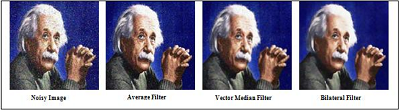
\includegraphics{10.png}

 Quality Measures of Einstein image
\end{center}

 A modified bilateral filtering method is implemented in this paper, which can effectively removed both impulsive noise and additive noise. Moreover MSE and PSNR of this method is the best.
